\subsubsection{Translator}
Translator klassen, oversætter spillet. Man vælger sproget som skal oversættes til ved at indtaste det som et program argument når man starter spillet (CLI). Man kan vælge mellem de sprog som ligger i resources mappen. Heri ligger der tekstfiler, der hedder det sprog som den indeholder. Spillet er blevet delvist oversat til engelsk, udover dansk. Klassen indlæser den fil som har det givne navn. 

\begin{figure}[H]
    \centering
    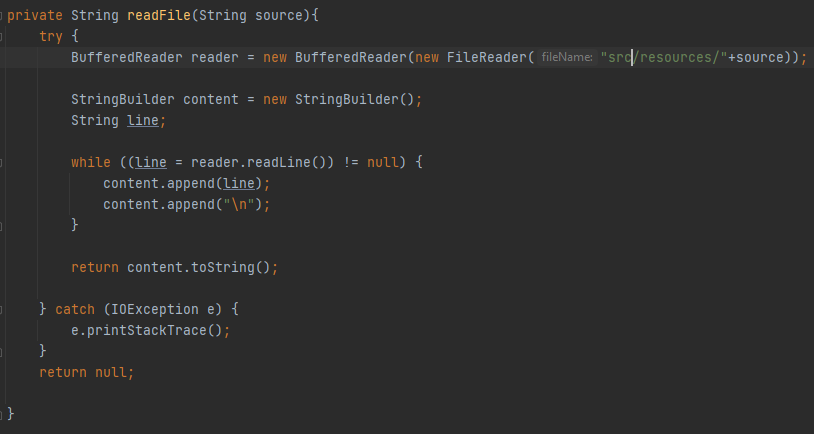
\includegraphics[width=\textwidth]{sources/7_implementering/readFileTranslator.PNG}
    \caption{readFile metoden i Translator klassen}
    \label{fig:readFile}
\end{figure}